%%%%%%%%%%%%%%%%%%%%%%%%%%%%%%%%%%%%%%%%%
% Contract
% LaTeX Template
% Version 1.0 (December 8 2014)
%
% This template has been downloaded from:
% http://www.LaTeXTemplates.com
%
% Original author:
% Brandon Fryslie
% With extensive modifications by:
% Vel (vel@latextemplates.com)
%
% License:
% CC BY-NC-SA 3.0 (http://creativecommons.org/licenses/by-nc-sa/3.0/)
%
% Note:
% If you are using Apple OS X, go into structure.tex and uncomment the font
% specifications for OS X and comment out the default specifications - this will
% drastically increase how good the document looks. You will now need to
% compile with XeLaTeX.
%
%%%%%%%%%%%%%%%%%%%%%%%%%%%%%%%%%%%%%%%%%

\documentclass[a4paper,12pt]{article} % The default font size is 12pt on A4 paper, change to 'usletter' for US Letter paper and adjust margins in structure.tex
\usepackage[francais]{babel}
%%%%%%%%%%%%%%%%%%%%%%%%%%%%%%%%%%%%%%%%%
% Contract
% Structural Definitions File
% Version 1.0 (December 8 2014)
%
% Created by:
% Vel (vel@latextemplates.com)
% 
% This file has been downloaded from:
% http://www.LaTeXTemplates.com
%
% License:
% CC BY-NC-SA 3.0 (http://creativecommons.org/licenses/by-nc-sa/3.0/)
%
%%%%%%%%%%%%%%%%%%%%%%%%%%%%%%%%%%%%%%%%%

%----------------------------------------------------------------------------------------
%	PARAGRAPH SPACING SPECIFICATIONS
%----------------------------------------------------------------------------------------

\setlength{\parindent}{0mm} % Don't indent paragraphs

\setlength{\parskip}{2.5mm} % Whitespace between paragraphs

%----------------------------------------------------------------------------------------
%	PAGE LAYOUT SPECIFICATIONS
%----------------------------------------------------------------------------------------

\usepackage{geometry} % Required to modify the page layout

\setlength{\textwidth}{16cm} % Width of the text on the page
\setlength{\textheight}{24.5cm} % Height of the text on the page

\setlength{\oddsidemargin}{0cm} % Width of the margin - negative to move text left, positive to move it right

% Uncomment for offset margins if the 'twoside' document class option is used
%\setlength{\evensidemargin}{-0.75cm} 
%\setlength{\oddsidemargin}{0.75cm}

\setlength{\topmargin}{-1.25cm} % Reduce the top margin

%----------------------------------------------------------------------------------------
%	FONT SPECIFICATIONS
%----------------------------------------------------------------------------------------

% If you are running Apple OS X, uncomment the next 4 lines and comment/delete the block below, you will now need to compile with XeLaTeX but your document will look much better

%\usepackage[cm-default]{fontspec}
%\usepackage{xunicode}

%\setsansfont[Mapping=tex-text,Scale=1.1]{Gill Sans}
%\setmainfont[Mapping=tex-text,Scale=1.0]{Hoefler Text}

%-------------------------------------------

\usepackage[utf8]{inputenc} % Required for including letters with accents
\usepackage[T1]{fontenc} % Use 8-bit encoding that has 256 glyphs

\usepackage{avant} % Use the Avantgarde font for headings
\usepackage{mathptmx} % Use the Adobe Times Roman as the default text font together with math symbols from the Sym­bol, Chancery and Com­puter Modern fonts

%----------------------------------------------------------------------------------------
%	SECTION TITLE SPECIFICATIONS
%----------------------------------------------------------------------------------------

\usepackage{titlesec} % Required for modifying section titles

\titleformat{\section} % Customize the \section{} section title
{\sffamily\large\bfseries} % Title font customizations
{\thesection} % Section number
{16pt} % Whitespace between the number and title
{\large} % Title font size
\titlespacing*{\section}{0mm}{7mm}{0mm} % Left, top and bottom spacing around the title

\titleformat{\subsection} % Customize the \subsection{} section title
{\sffamily\normalsize\bfseries} % Title font customizations
{\thesubsection} % Subsection number
{16pt} % Whitespace between the number and title
{\normalsize} % Title font size
\titlespacing*{\subsection}{0mm}{5mm}{0mm} % Left, top and bottom spacing around the title % Input the structure.tex file which specifies the document layout and style
\usepackage{graphicx}
%----------------------------------------------------------------------------------------
%	DYNAMIC CONTRACT INFORMATION
%----------------------------------------------------------------------------------------

% Your name and company name
\newcommand{\YourName}{Jean LAPOSTOLLE et Lucas LEROY}
\newcommand{\CompanyName}{ORAY Corp.}

% Your address
\newcommand{\AddressLineOne}{127 rue de la route}
\newcommand{\AddressLineTwo}{80000, Amiens}

% Your email address
\newcommand{\YourEmail}{service.client@oray.fr}

% The client's name
\newcommand{\ClientName}{Projet corp.}

% The delivery date for specifications and completion date for the project
\newcommand{\DeliveryDate}{25 Janvier 2018}
\newcommand{\CompletionDate}{19 Avril 2018}


% Payee's information
\newcommand{\PayeeName}{ORAY corp.}
\newcommand{\PaymentAddressLineOne}{127 rue de la route}
\newcommand{\PaymentAddressLineTwo}{80000}
\newcommand{\PaymentAddressLineThree}{Amiens}

%----------------------------------------------------------------------------------------

\begin{document}

%----------------------------------------------------------------------------------------
%	TITLE PAGE
%----------------------------------------------------------------------------------------

\begin{titlepage}

\vspace*{\fill} % Add whitespace above to center the title page content

\begin{center}

{\LARGE Cahier des Charges pour le logiciel de \ClientName~}\\ [1.5cm]

Soumis le: \today

\end{center}

\CompanyName\\

\YourName\\

\AddressLineOne

\AddressLineTwo

\YourEmail

\vspace*{\fill} % Add whitespace below to center the title page content

\end{titlepage}

%----------------------------------------------------------------------------------------
%	OBJECTIVE SECTION
%----------------------------------------------------------------------------------------

\section{Objectifs}

\YourName~(mentionnés ci-après comme les développeurs) est engagé par \ClientName~(mentionné ci-après comme le client)
dans le projet de création d'un logiciel/site web de calcul scientifique(mentionné ci après comme la calculatrice). Le site Web sera hébergé
par le client.
Le projet a pour but, auprès du client, de proposer librement un service Web et un service logiciel de calcul scientifique à ceux qui
souhaite une calculatrice fonctionnelle et intuitive.
%----------------------------------------------------------------------------------------
%	DELIVERABLES SECTION
%----------------------------------------------------------------------------------------


Le client souhaitant répondre à la problèmatique du calcul scientifique libre, le produit devra répondre à minima aux besoins suivant:
\begin{itemize}
  \item Gestion des fonctions mathématiques de base.
  \item Gestion de l'affichage graphique de fonctions
  \item Résolution d'équation jusqu'au second degré
  \item Gestion d'un historique des calculs
  \item L'enregistrement de sessions de calculs
\end{itemize}
 De plus une documentation utilisateur de la calculatrice devra être accessible.



\section{Interface Graphique}

Afin d'offrir une expérience utilisateur similaire aux offres existantes comme les calculatrices physiques ou un outils en ligne comme Wolfram Alpha, le logiciel 
comprends une entrée utilisateur permettant d'écrire le calcul en notation infixée classique. ex: $$ (127 + 3) / 2 + 5 $$

L'historique des calculs déjà effectués se fera en dessous de l'entrée utilisateur du plus récent au plus ancien. Les résultats pourront être réutilisées en cliquant
dessus. 

La calculatrice possède un menu d'import/export de l'historique ce qui permet de sauvegarder/charger des sessions de calculs.
Le menu contient aussi le lien vers la documentation de la calculatrice. Chaque fonction de la calculatrice y est détaillé (Nom, implémentation, syntaxe, exemple).

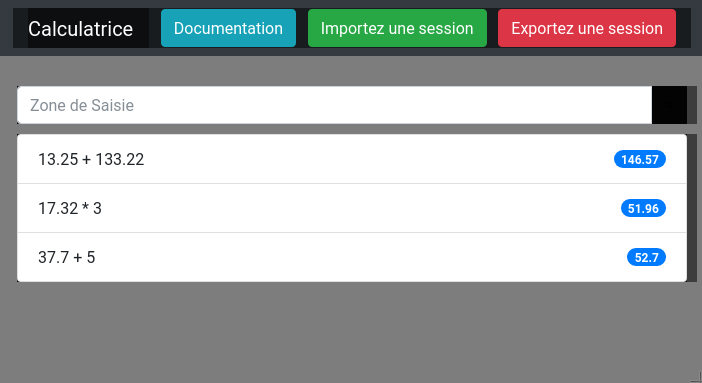
\includegraphics[scale=0.7]{visual.png}




%----------------------------------------------------------------------------------------
%	SCHEDULE SECTION
%----------------------------------------------------------------------------------------

\section{Termes du contrat}

Le projet devra être accompli avant le \CompletionDate.

%----------------------------------------------------------------------------------------
%	TERMS AND CONDITIONS SECTION
%----------------------------------------------------------------------------------------

\section{Conditions}
\subsection{Hébergement}
L'hébergement est à la charge du client, mais un manuel de mis en production devra être livré au client. 
Les développeurs devront prendre en compte la surcharge du serveur, notamment, en laissant la machine utilisateur faire les calculs.

\subsection{Performance}
Les performances de la calculatrice ne sont pas pris en compte, cependant un temps raisonnable est attendu, au moins pour les calculs basiques.

\subsection{Maintenance}
La maintenance de la calculatrice ne fait pas partie du présent contrat. Un éventuel nouveau contrat pourrait être engagé, à la 
suite des résultats de celui-ci, concernant la maintenance.

\subsection{Limites de la calculatrice}
Les limites de la calculatrice sont:
\begin{itemize}
  \item La capacité des nombres est limité à la taille mémoire de la machine.
  \item La précision du nombre est rentré par l'utilisateur, par défaut est de 6 chiffres après la virgule.
  \item Les constantes classiques seront enregistrées dans la calculatrice avec une précision d'au moins une centaine de chiffres après la virgule.
\end{itemize}

\subsection{Accessibilité}
Le site web et le logiciel étant produits à un usage scientifique devra être accessible à une personne ayant une affinité avec la science, à partir du lycée.

Les normes d'accessibilité international WCAG 2.0 doivent être respecté.


\subsection{Format}
Le logiciel doit fonctionné sur les plate-formes Windows, Linux et MacOS.
Le site web doit être compatible avec les navigateurs Google Chrome, Chromium, Mozilla Firefox et Opéra.


\section{Description détaillé du besoin}

\subsection{Saisie Utilisateur}
La saisie Utilisateur se fera à partir d’un clavier d’ordinateur, en notation infixée classique.
$$ (3+5)*2 + cos(5*PI) $$


\subsection{Gestion des fonctions de base}
Les fonctions basique de style $* / + - l^{x} \sqrt{x}$ doivent être calculées. Les fonctions de trigonométries 
classique aussi, tels que cos, sin, tan, arctan, arccos, arcsin, ln, log, exp. Possibilités d’affectation de variables.

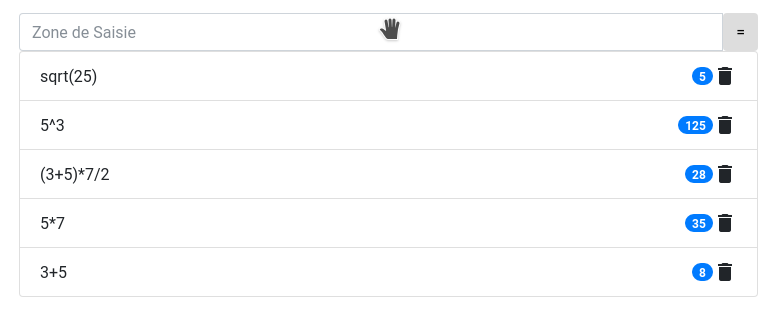
\includegraphics[height=4cm]{fctbase.png}

\subsection{Affichage de graphique}
 Affichage de fonctions graphiques 2D et 3D.

 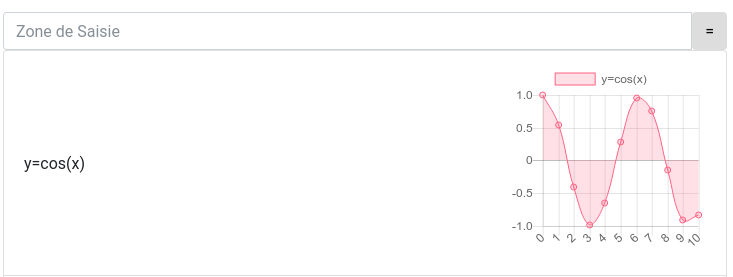
\includegraphics[height=4cm]{graph.png}

\subsection{Gestion de  la mémoire}
Historique des calculs et des résultats. Réutilisation. Enregistrement dans un journal de session.

\subsection{Gestion des équations}
Résolution d’une équation jusqu’aux équations de degré 3.

 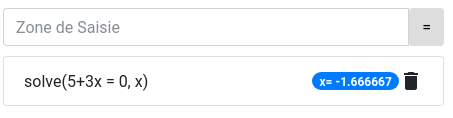
\includegraphics[height=2cm]{fctsolve.png}

\subsection{Gestion des erreurs}
Affichage des erreurs rencontrées lors de l’exécution de l’algorithme. Typiquement lors d'une ``/0''. La distinction des erreurs devra être faite pour permettre à
 l'utilisateur de comprendre son erreur.


\subsection{Documentation}
Création d’une documentation contenant la pré-condition, la post-condition, la syntaxe, l'implémentation et quelques exemples de chaque fonction.

\subsection{Auto-complétion}
Lors de la saisie, l’utilisateur doit avoir une auto-complétion des fonctions, avec une aide sur les arguments de la fonction.

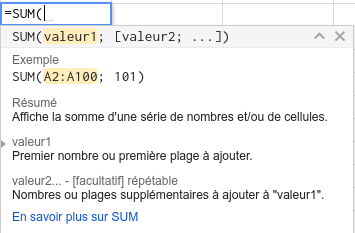
\includegraphics[height=4cm]{autocomplete.png}

\subsection{Bonus}

\subsubsection{Gestion des matrices}
Fonctions basiques de matrices $ + - * l^{x} $. Linéarisation par Gauss. Gestion de l ‘entrée utilisateur. Déterminant,
inverse, transposé, pseudo-inverse.

\subsubsection{Gestion du calcul différentiel}
Dérivation, intégration (restreint à un certains cadre).

\subsubsection{Gestions des nombres complexes}
Entrées des nombres complexes. Changement de formes des nombres. Calcul de modules et d’argument.









%----------------------------------------------------------------------------------------
%	ACCEPTANCE SECTION
%----------------------------------------------------------------------------------------

\newpage % Put signatures on a separate page

\section{Approbation}

Tous changements du présent contrat sera soumis à l'acceptation des deux parties.

Les signatures suivantes sont témoins de l'acceptation du présent contrat par les deux parties aux dates indiquées.
%------------------------------------------------

\subsection*{Le Client} % Suppress section numbering with the *

\ClientName \\

\begin{tabular}{lp{10pt}l}
Signature: && \hspace{0.5cm} \makebox[3in]{\hrulefill} \\ \\[3pt]
Nom (en lettres moulées): && \hspace{0.5cm} \makebox[3in]{\hrulefill} \\ \\[3pt]
Titre: && \hspace{0.5cm} \makebox[3in]{\hrulefill} \\ \\[3pt]
Date: && \hspace{0.5cm} \today
\end{tabular}

%------------------------------------------------

\subsection*{Les Développeurs} % Suppress section numbering with the *

\YourName \\

\begin{tabular}{ l p{10pt} l }
Signatures: && \hspace{0.5cm} \makebox[3in]{\hrulefill} \\ \\[3pt]
Noms (en lettres moulées): && \hspace{0.5cm} \makebox[3in]{\hrulefill} \\ \\[3pt]
Titre: && \hspace{0.5cm} \makebox[3in]{\hrulefill} \\ \\[3pt]
Date: && \hspace{0.5cm} \today
\end{tabular}

%----------------------------------------------------------------------------------------

\end{document}
